
\section{Existing ontology work}
\label{existingontologies}

One of the key aspects of FAIR ontologies is that they are reusable and profit
from the reusability of existing ontologies \cite{PovedaVillalon.2020}. We did
an extensive analysis of existing ontologies with infrastructure, charging
stations, electric vehicles and electricity grid in scope. We also rely
strongly on the review performed by Katsumi and Fox regarding transport
planning vocabularies \cite{Katsumi.2018}. In this section we summarize the
ontologies we considered for reutilization and justify the situations in which
we decide not to reutilize existing concepts.


\subsection{The Open Energy Ontology}

The OEO has been in active development since 2021 with several releases since
then. It exists to address a technical gap associated with knowledge management
in the field of energy systems analysis. Said gap is the lack of common
semantics to annotate and share datasets and tools associated with the
mentioned discipline. The ontology is part of a larger data ecosystem called
the Open Energy Family (OEF), which allows researchers to share data sources
and results in accordance with the FAIR principles. It has had moderate
success, particularly within the context of projects associated to the OEF such
as the Open Energy Platform (OEP) \cite{Hulk.2024}. One of the characteristics
that makes this and other FAIR ontologies transparent and accessible is the
fact that it is being openly developed in a shared
repository\footnote{https://github.com/OpenEnergyPlatform/ontology}. An
important work on the inclusion of concepts coming from the transport sector
was performed by \cite{Mittermeier.2023}, who did several implementations
associated to the topic. However since the size of the task is larger than what
can be achieved during a master thesis, many implementations were left open in
the form of GitHub Issues. In some of these issues it was made clear that the
scope of the OEO is in some cases beyond what is often necessary to represent
phenomena in the transport sector.


In our charging infrastructure ontology we need a way of describing vehicles,
particularly electric vehicles. The OEO has a rich taxonomy of vehicles that
rest on the definition of artificial objects which are in the context of BFO
`causally unified material entities deliberately manufactured by humans to
address a particular porpoise'. The taxonomy has multiple parallel
ramifications, one associated to its energy consumption mode like `electric
vehicle', `internal combustion vehicle' and `gas turbine vehicle' and another
associated to its operational medium such as `land vehicle', `aircraft' or
`watercraft'. The former has axiomatization significant for electric grid and
energy systems models which can be seen in figure \ref{evcommitments} the
latter lacks its own axioms and relies on mainly on the former. To our
application is only interesting to use the taxonomy of electric vehicles
(Figure \ref{evtax}). Its land vehicle taxonomy is very rich (figure
\ref{landvehicletaxoeo}) and contains elements that might have conflicts with
any future implementation in a transport ontology. Because of this we rely on
the Common Core Ontologies (CCO), this will be clarified in its respective
section.


\begin{figure}[h]\label{evtax}
    \caption{Open energy ontology electric vehicle taxonomy.}
    \centering
    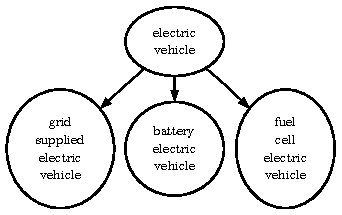
\includegraphics[width=0.6\textwidth]{images/OEOVehicles}
\end{figure}

\begin{figure}[h]\label{evcommitments}
    \caption{Open energy ontology electric vehicle commitments.}
    \centering
    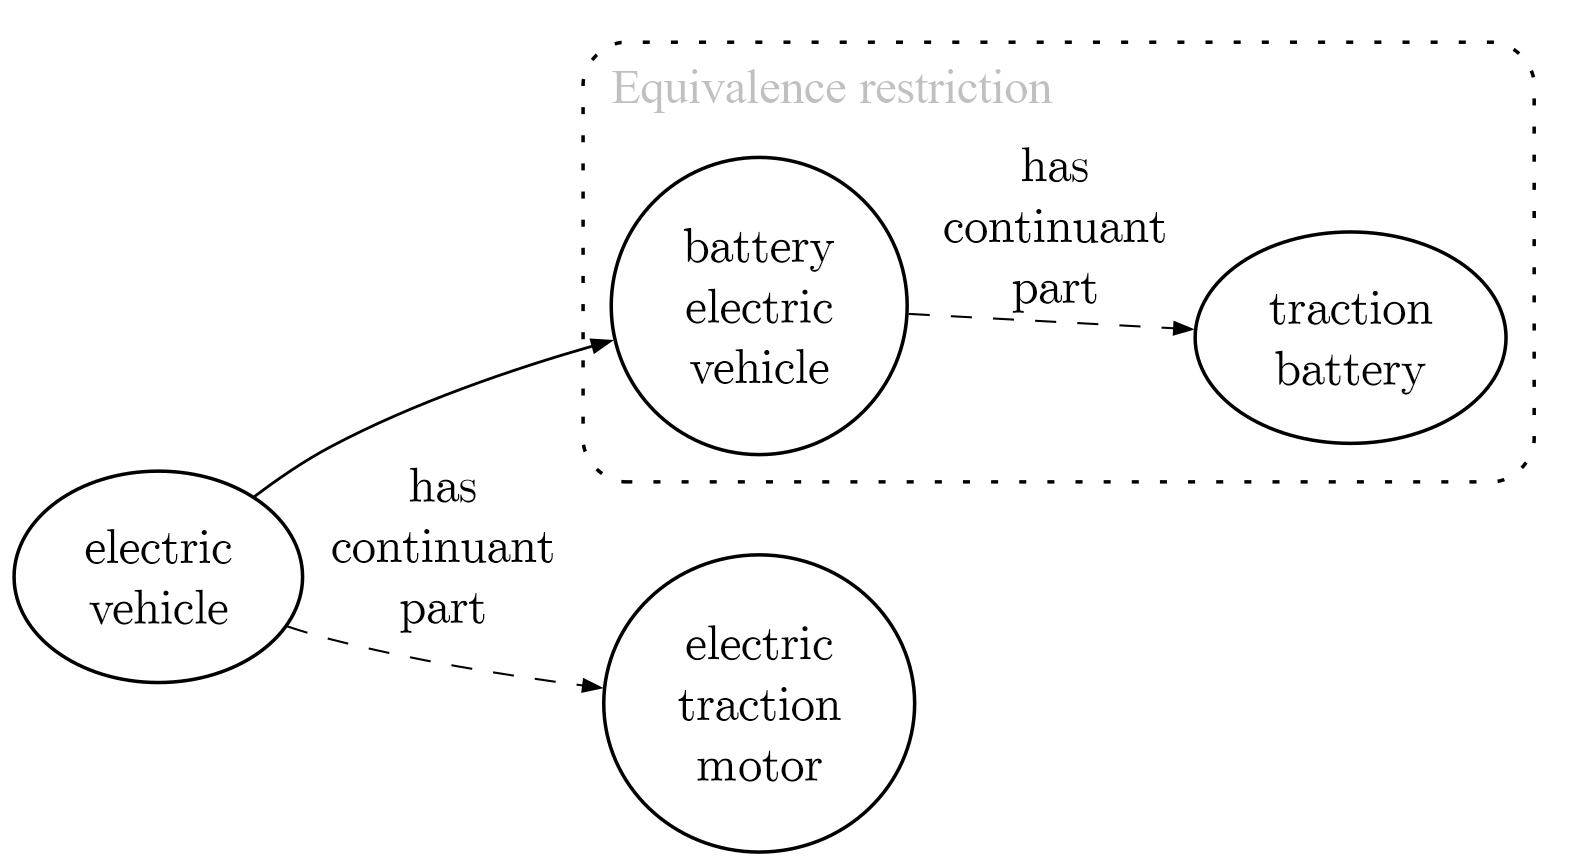
\includegraphics[width=0.9\textwidth]{images/OEOEV}
\end{figure}


\subsection{The Common Core Ontologies}

CCO section keywords: Infrastructure, Facilities Vehicle taxonomy

\begin{figure}[h]\label{landvehicletaxoeo}
    \caption{OEO Vehicle Taxonomy.}
    \centering
    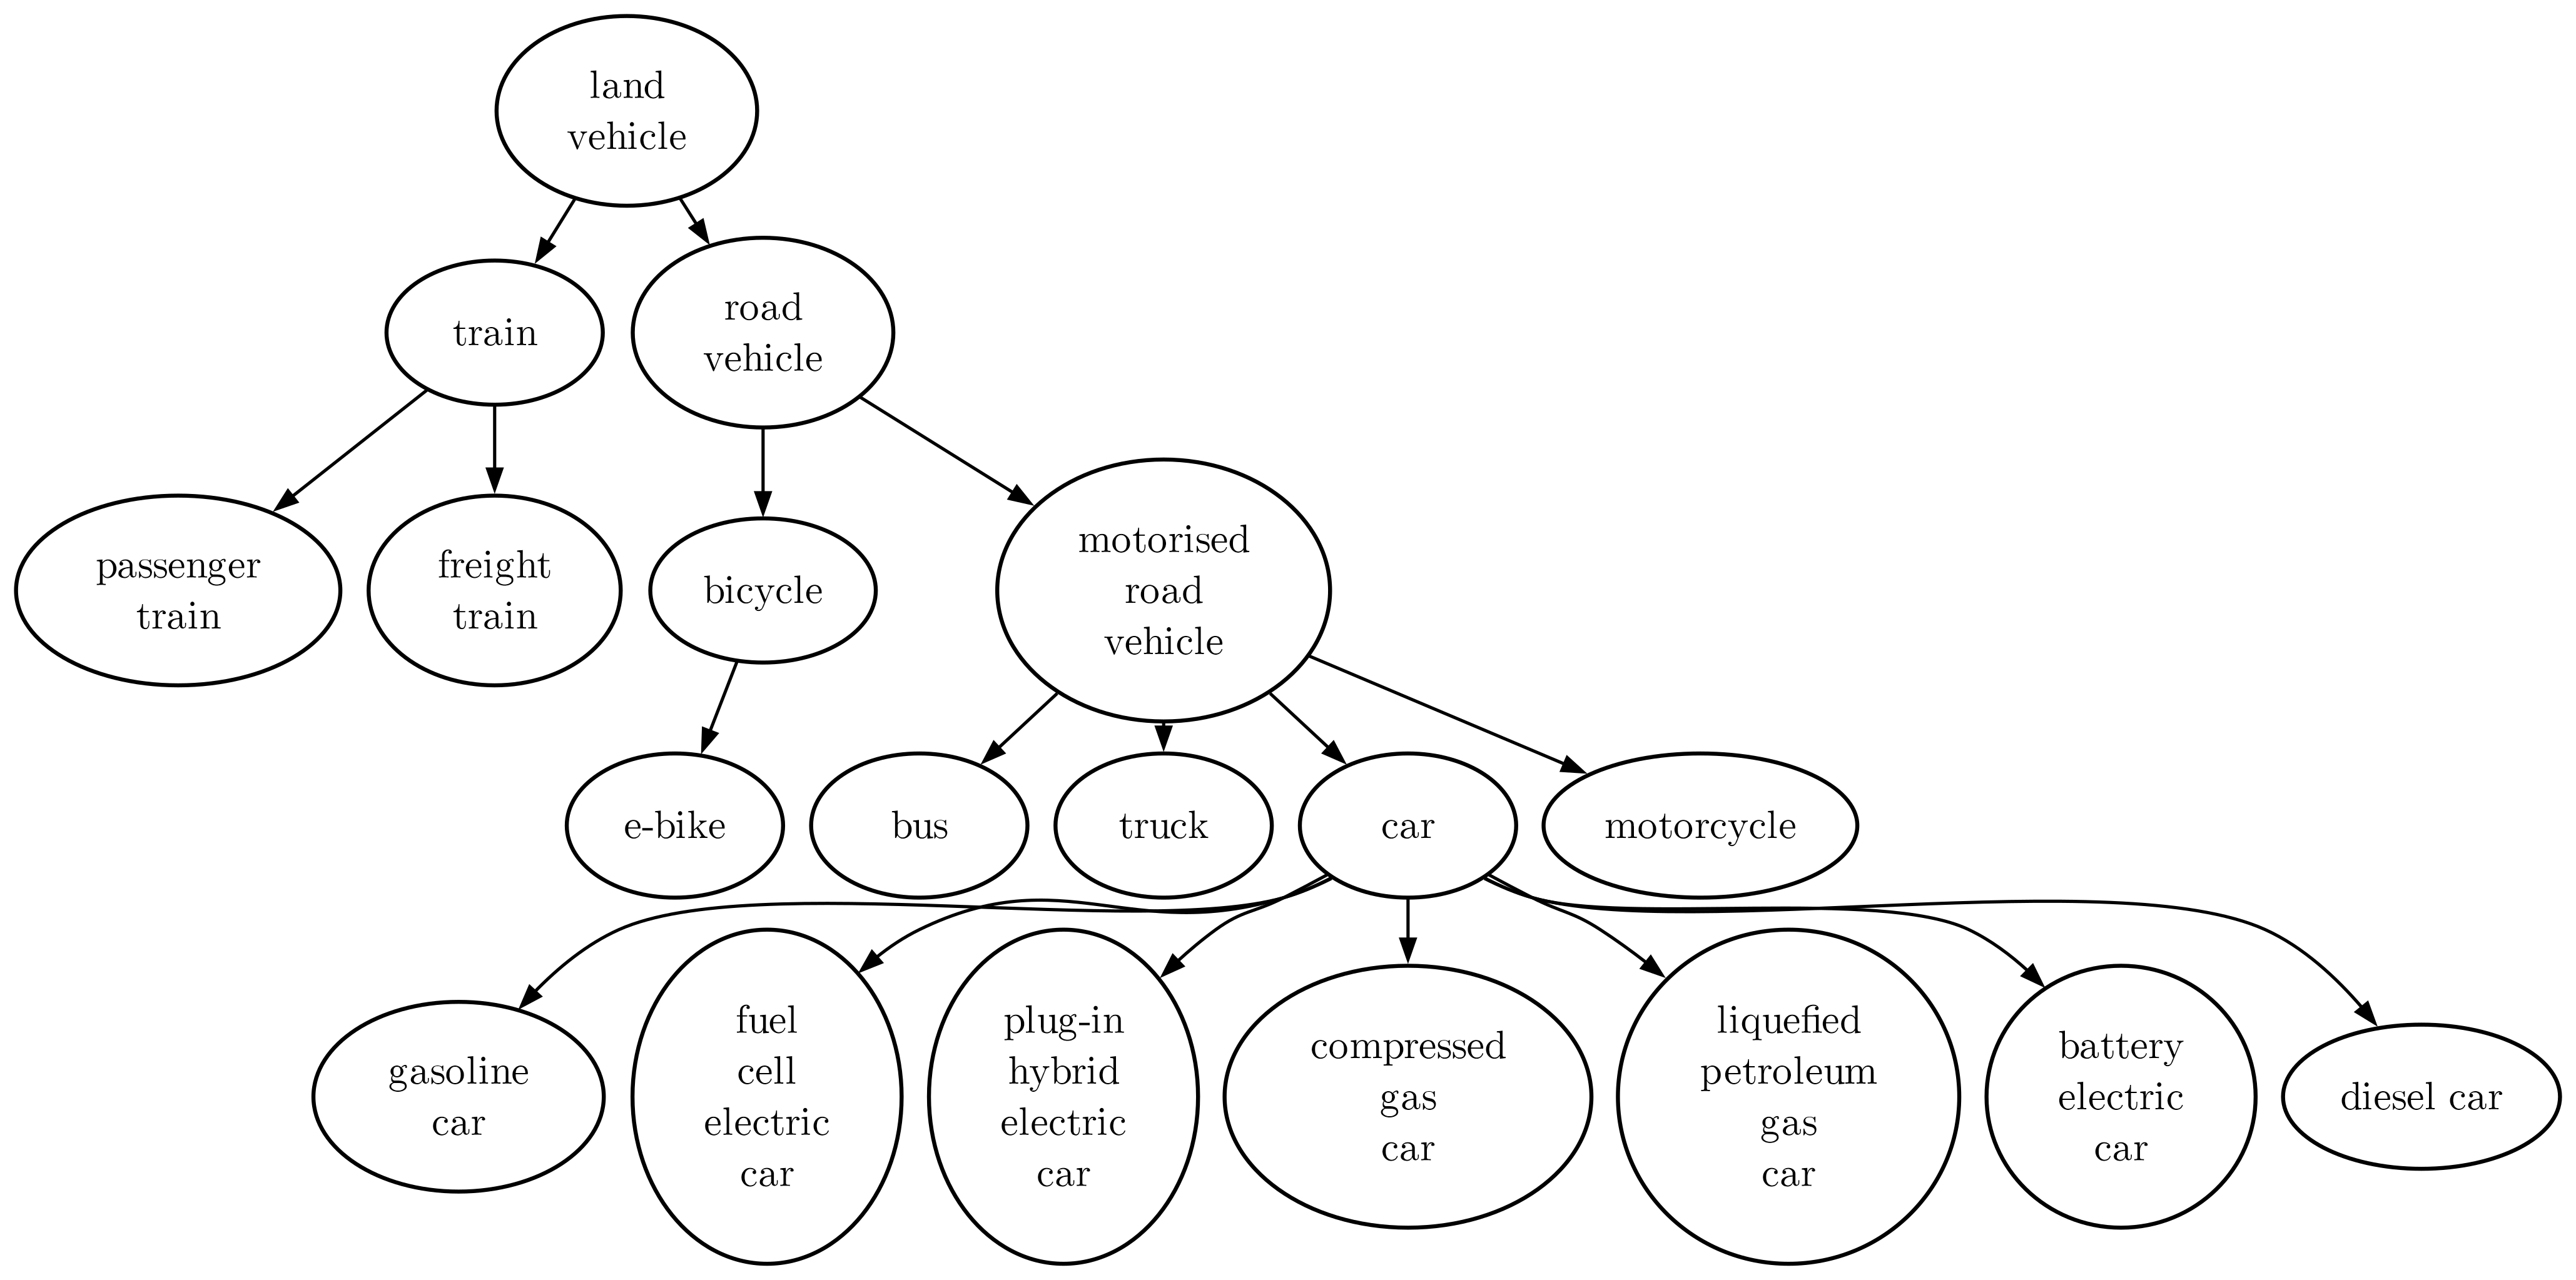
\includegraphics[width=0.9\textwidth]{images/OEOLVehicles}
\end{figure}

\begin{figure}[h]
    \caption{Common Core Ontologies Vehicle Taxonomy.}
    \centering
    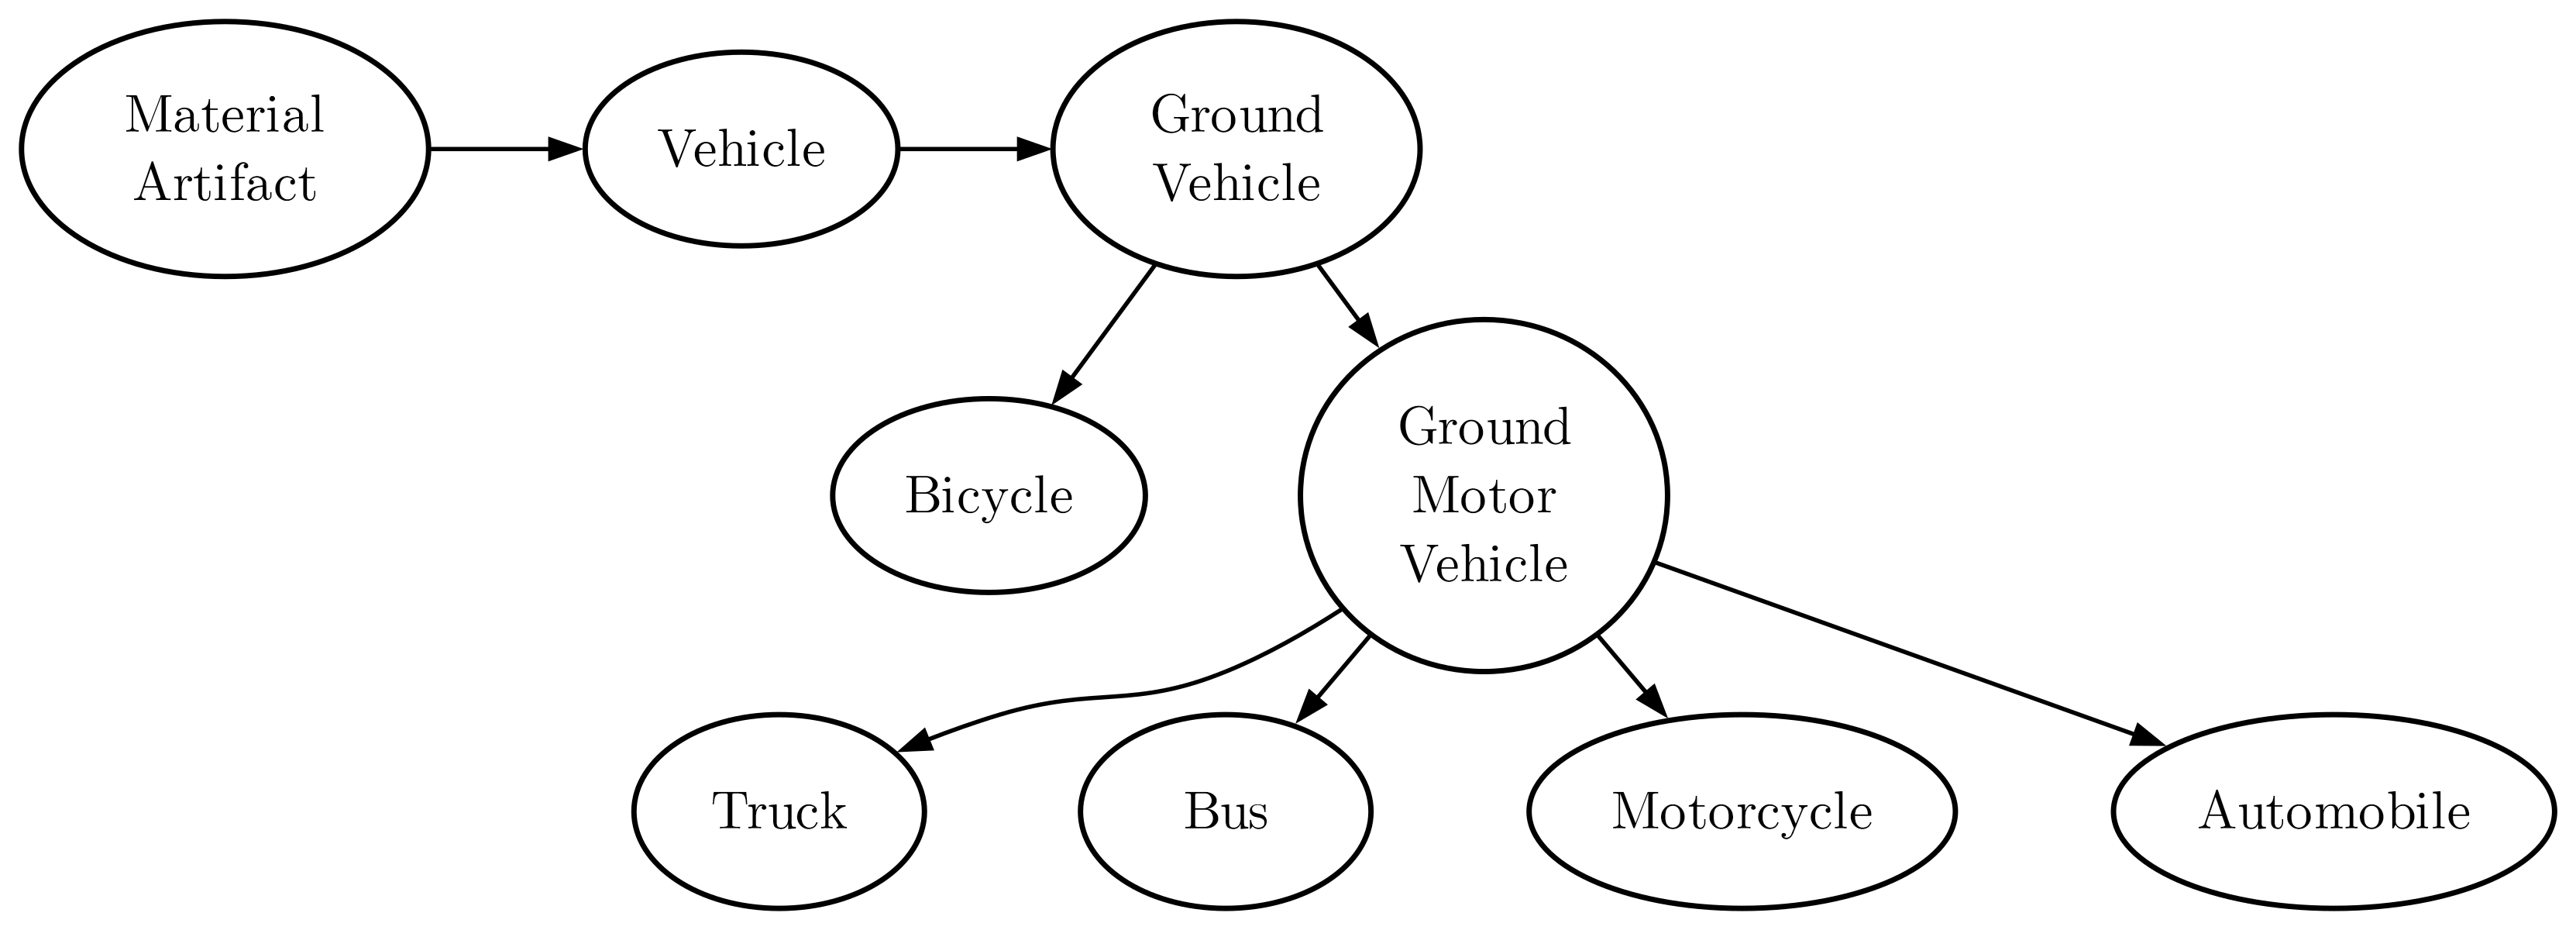
\includegraphics[width=0.9\textwidth]{images/CCOVehicles}
\end{figure}


\begin{figure}[h]
    \caption{Common Core Ontologies infrastructure constraints.}
    \centering
    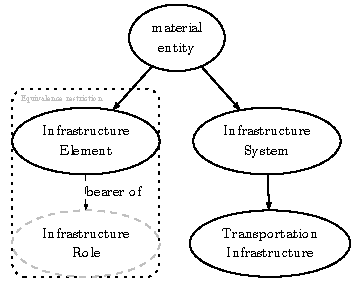
\includegraphics[width=1.0\textwidth]{images/infrastructureSystem}
\end{figure}



\subsection{iCity Parking ontology}

Parking section, keywords: Application specific, different Spatio-temopral assumptions

\begin{figure}[h]
    \caption{iCity parking ontology commitments associated to charging infrastructure.}
    \centering
    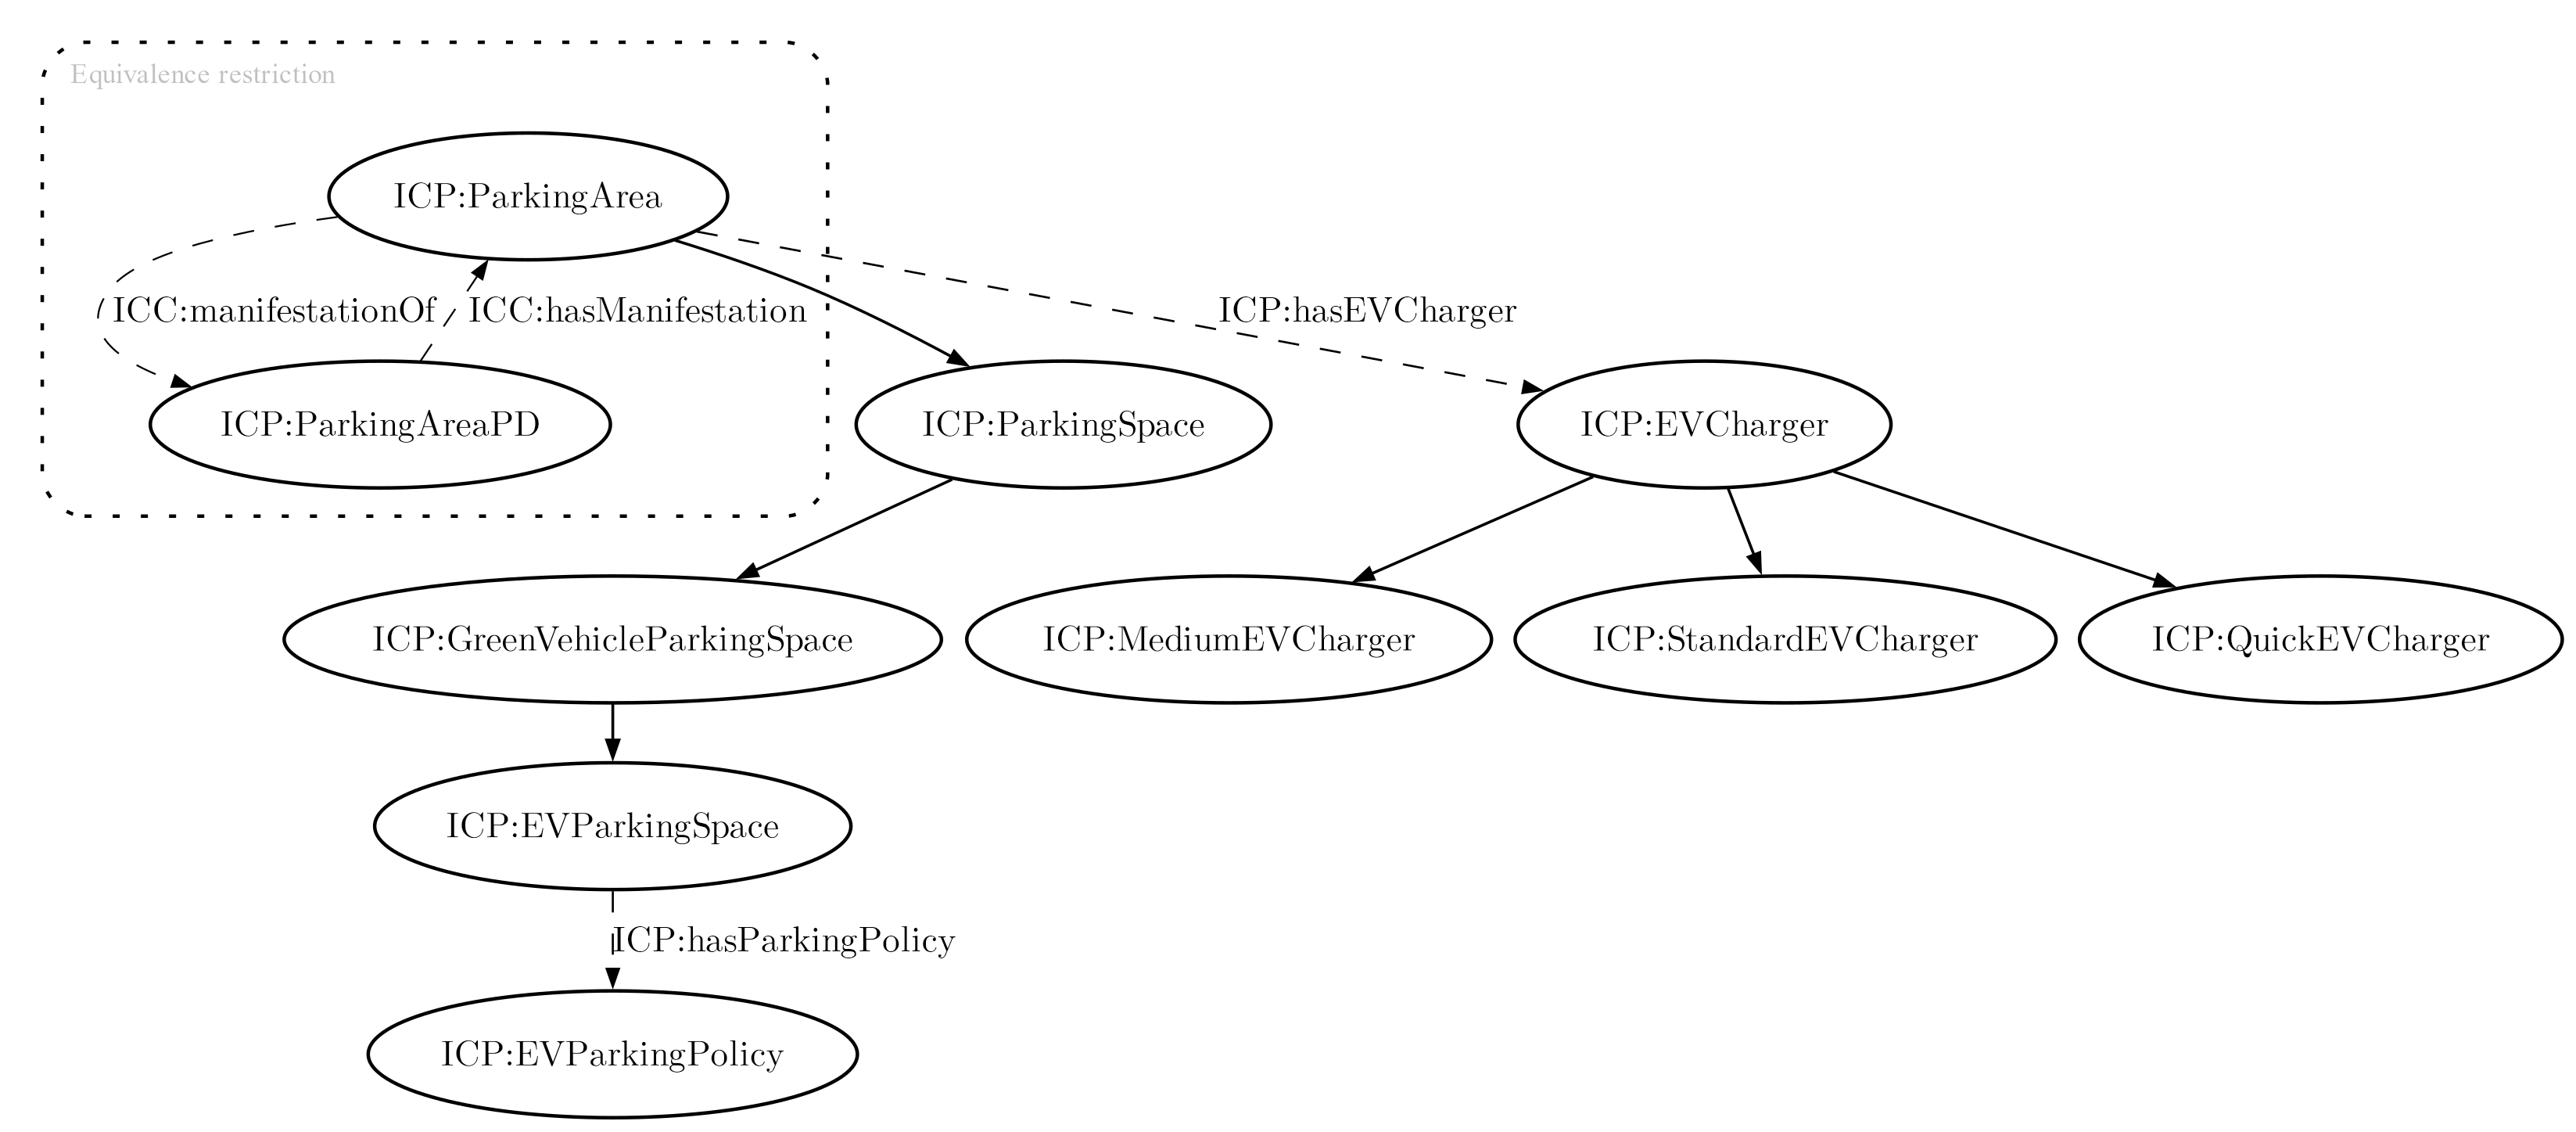
\includegraphics[width=1.0\textwidth]{images/PARKING}
\end{figure}

\subsection{The virtues of using Upper Level Ontologies}
\label{upperlevel}


\subsubsection{The Basic Formal Ontology}

BFO has its own mereology where objects ocupying the same spatiotemporal place
are the same. BFO is bad for materials because it does not consider constitution.
BFO has advantages in regards to object aggreagates, it is relatively easy to represent
membership with it. 
